%!TEX root = proj_report_outline.tex
\chapter{Conclusions and Future Work}
This chapter reviews the project's contributions in light of the design requirements, discusses potential future work and finally, surmises the project.

\section{Review}\label{S:review}

The project's principal contributions are as follows:

\paragraph{C1:} I have developed an {\em Innovation Role Taxonomy} for classifying existing innovation platforms. The relationship semantics between roles in the taxonomy is denoted as either explicitly supported or implicitly supported. Platforms that facilitate innovation collaboration ideally have explicit support for all roles.

\paragraph{C2:} I have designed a {\em new UI} to encourage collaboration and be visually appealing. Content templates and wire frames were key artefacts produced to guide the final implementation.

\paragraph{C3:} I have designed the {\em PitchHub distributed architecture}. The tiered architecture style adopted supports ease of extension for future development.

\paragraph{C4:} I have developed {\em the first suite of user stories} that capture the interactions of innovation collaboration. These stories specify the following: engagement of all roles within the innovation community, the ability to scope content's disclosure, and audit who has seen ideas that you have initiated.

\paragraph{C5:} I have implemented the {\em PitchHub prototype}, a platform that supports the innovation collaboration user stories specified. Built on the Ruby on Rails framework and by using good coding practices this artefact is open to future development.

\paragraph{C5.1:} I have {\em deployed a PitchHub prototype} to Callaghan Innovation for their use. This instance contains the following production configuration: a Passenger application server, caching, SSL, and various security measures suggested by OWASP (e.g. ssh hardening, protection against IP spoofing). Visit \url{http://pitchhub.net} to view this instance.


\paragraph{C5.2:} I have extended the {\em PitchHub prototype with Shamir's Secret Sharing scheme}. Sensitive information such as Pitch Points, suggestions, and comments are encrypted using this service.

\paragraph{C5.3:} I have extended the {\em PitchHub prototype with diverse secret keepers} to strengthen the security provided by the Secret Sharing scheme. The prototype supports the following databases: MongoDB, Postgres, MySQL and SQLite. To maintain the \textit{plug-and-play} functionality afforded by MongoDB the configuration required by SQL secret keepers has been automated.

\paragraph{C6:} I have virtualised the {\em PitchHub development environment} using Vagrant and Chef to make installation and setup of PitchHub as easy as possible. This was primarily for the benefit of non-technical stakeholders, but will be equally useful for future maintainers.

\paragraph{C7:} I have automated the {\em PitchHub deployment process} using Capistrano to make host configuration and code deployment as easy as possible. The scripts defined facilitate zero-downtime deployments and also enable deployments to be rolled-back easily.
\\
\newline
These contributions are instrumental in fulfilling the design requirements identified in Section \ref{S:designRequirements}. The fulfilment relationship between contributions to requirements is shown in Figure \ref{fig:contribution_requirements_mapping}.

\begin{figure}[ht]
    \centering
    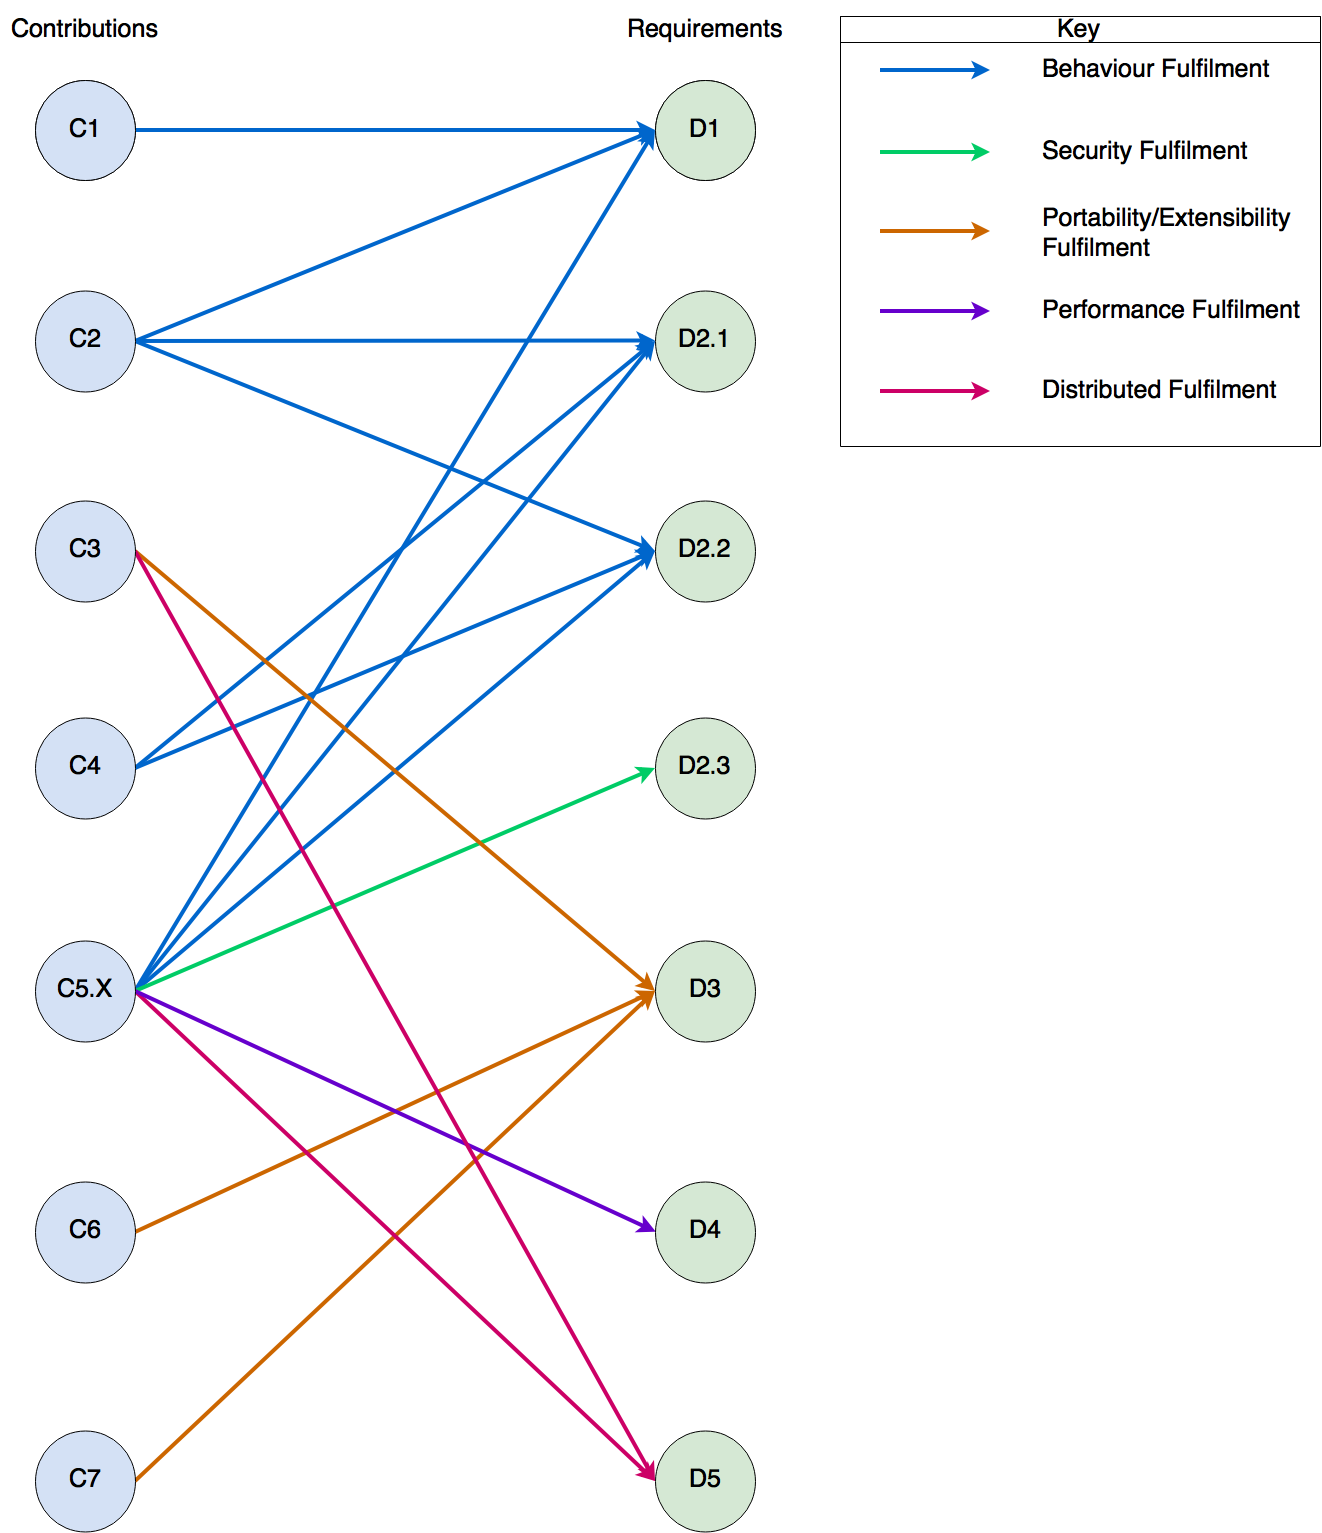
\includegraphics[width=0.65\textwidth]{contributions_requirements_map}
    \caption{A mapping of contributions to requirements denoting fulfilment.}
    \label{fig:contribution_requirements_mapping}
\end{figure}

The blue mapping in Figure \ref{fig:contribution_requirements_mapping} demonstrates the fulfilment of the behaviour orientated requirements: D1, D2.1, and D2.2. The user stories created in C1 capture the behaviours required by D1, D2.1, and D2.2. These user stories were used to drive the design process of the UI (C4) that C5.{\em X} ultimately uses to facilitate these behaviours. The strict adherence to the user stories throughout the design and execution of the project has culminated in artefacts that are faithful in their support of the behaviours required. This fulfilment has been verified by Test \rom{1} and thus requirements D1, D2.1, and D2.2 are concluded as fulfilled.

The green mapping in Figure \ref{fig:contribution_requirements_mapping} represents C5.3 and C5.4's contributions to the fulfilment of the security requirement, D2.3. Integrating the Secret Sharing scheme into the prototype and encrypting commercially sensitive data and IP at the Pitch Point level ensures unconditional security in relation to database breaches (of up to \textit{k}). As described in Section \ref{S:evaluationScope} verification of this component was out of scope of this project. Despite this, it is believed that requirement D2.3 has been fulfilled to the extent possible within the scope of this project.

The orange mapping in Figure \ref{fig:contribution_requirements_mapping} demonstrates the fulfilment of the portability/extensibility requirement, D3. The architecture (C3) aids extensibility through the tiered architecture style adopted. The virtualised development environment (C6) is key in providing portability, enabling \textit{plug-and-play} functionality for all artefact prototype variations (C5.{\em X}). C7 aids in the extensibility of the deployment process, as new tasks and environment targets can be easily added.

The purple mapping in Figure \ref{fig:contribution_requirements_mapping} reflects the fulfilment of the performance requirement (D4). This was verified on C5.{\em X} through the Tests \rom{3}-\rom{6}. Specifically, Tests \rom{3}-\rom{5} verified that the main flows can be performed within Nielsen's time thresholds (in different Secret Sharing configurations) and Test 6 verified that the prototype can sustain the expected community size's load while maintaining the mean response wall-time within the time thresholds. Therefore, in the context of Nielsen's response time thresholds requirement D4 has been met.

The pink mapping in Figure \ref{fig:contribution_requirements_mapping} showcases the fulfilment of the distributed requirement, D5. C3 demonstrates the distributed architecture PitchHub is built upon in satisfaction of requirement D5. Ultimately through C5.3 and C5.4's verification of C3's design in their implementation and evaluation it is concluded that requirement D5 has been satisfied.

\section{Future Work}

This section discusses potential extensions to the PitchHub prototype.

\subsection{Recommendation Engine}

A potentially useful feature would be if Pitch Cards could be recommended to users based on their ontological profile. This would encourage collaboration through showing users ideas they are more likely to have an interest in. Offline learning is certainly viable, but an interesting challenge would be integrating the recommender to work with the Secret Sharing service in an online learning approach.

\subsection{Usability Extension/Evaluation}

Future work concentrating on the usability of PitchHub could focus on evaluating and extending the current prototype. A user study would be beneficial in verifying the accuracy of the behaviours identified in the user stories. A user study could also help with the identification of new user stories and potential functionality extensions. 

\subsection{RealMe Integration}

When PitchHub is released to the public it may be open to abuse by users creating fake accounts. These fake accounts may be used maliciously to view others' IP or contribute unhelpful suggestions. Therefore it is important for users on PitchHub to be verified as being who they say they are so that there may be a sense of accountability. A service like RealMe would be ideal for this as it is maintained by the Department of Internal Affairs and the actual identity verification process is facilitated by them. To integrate RealMe into PitchHub would require using RealMe's SAML service for authentication.

\section{Summary}

This project has produced and evaluated PitchHub, an online collaboration platform for the innovation community. PitchHub provides explicit collaboration support for all roles in the innovation community, enables users to audit/scope the dissemination of their content, and ensures that all potentially commercially-sensitive content is stored securely.

The evaluation of the prototype demonstrated two key aspects. First, that PitchHub can support the size of the New Zealand innovation community and second, that PitchHub satisfies Nielsen's response time thresholds (across all the configurations tested). 

Ultimately by having been accepted into Callaghan Innovation, the artefact produced was successful in it's aim of facilitating innovation collaboration.